% Options for packages loaded elsewhere
\PassOptionsToPackage{unicode}{hyperref}
\PassOptionsToPackage{hyphens}{url}
\PassOptionsToPackage{dvipsnames,svgnames,x11names}{xcolor}
%
\documentclass[
  12pt,
  legalpaperpaper,
  DIV=11,
  numbers=noendperiod]{scrartcl}

\usepackage{amsmath,amssymb}
\usepackage{iftex}
\ifPDFTeX
  \usepackage[T1]{fontenc}
  \usepackage[utf8]{inputenc}
  \usepackage{textcomp} % provide euro and other symbols
\else % if luatex or xetex
  \usepackage{unicode-math}
  \defaultfontfeatures{Scale=MatchLowercase}
  \defaultfontfeatures[\rmfamily]{Ligatures=TeX,Scale=1}
\fi
\usepackage{lmodern}
\ifPDFTeX\else  
    % xetex/luatex font selection
\fi
% Use upquote if available, for straight quotes in verbatim environments
\IfFileExists{upquote.sty}{\usepackage{upquote}}{}
\IfFileExists{microtype.sty}{% use microtype if available
  \usepackage[]{microtype}
  \UseMicrotypeSet[protrusion]{basicmath} % disable protrusion for tt fonts
}{}
\makeatletter
\@ifundefined{KOMAClassName}{% if non-KOMA class
  \IfFileExists{parskip.sty}{%
    \usepackage{parskip}
  }{% else
    \setlength{\parindent}{0pt}
    \setlength{\parskip}{6pt plus 2pt minus 1pt}}
}{% if KOMA class
  \KOMAoptions{parskip=half}}
\makeatother
\usepackage{xcolor}
\setlength{\emergencystretch}{3em} % prevent overfull lines
\setcounter{secnumdepth}{-\maxdimen} % remove section numbering
% Make \paragraph and \subparagraph free-standing
\ifx\paragraph\undefined\else
  \let\oldparagraph\paragraph
  \renewcommand{\paragraph}[1]{\oldparagraph{#1}\mbox{}}
\fi
\ifx\subparagraph\undefined\else
  \let\oldsubparagraph\subparagraph
  \renewcommand{\subparagraph}[1]{\oldsubparagraph{#1}\mbox{}}
\fi

\usepackage{color}
\usepackage{fancyvrb}
\newcommand{\VerbBar}{|}
\newcommand{\VERB}{\Verb[commandchars=\\\{\}]}
\DefineVerbatimEnvironment{Highlighting}{Verbatim}{commandchars=\\\{\}}
% Add ',fontsize=\small' for more characters per line
\usepackage{framed}
\definecolor{shadecolor}{RGB}{241,243,245}
\newenvironment{Shaded}{\begin{snugshade}}{\end{snugshade}}
\newcommand{\AlertTok}[1]{\textcolor[rgb]{0.68,0.00,0.00}{#1}}
\newcommand{\AnnotationTok}[1]{\textcolor[rgb]{0.37,0.37,0.37}{#1}}
\newcommand{\AttributeTok}[1]{\textcolor[rgb]{0.40,0.45,0.13}{#1}}
\newcommand{\BaseNTok}[1]{\textcolor[rgb]{0.68,0.00,0.00}{#1}}
\newcommand{\BuiltInTok}[1]{\textcolor[rgb]{0.00,0.23,0.31}{#1}}
\newcommand{\CharTok}[1]{\textcolor[rgb]{0.13,0.47,0.30}{#1}}
\newcommand{\CommentTok}[1]{\textcolor[rgb]{0.37,0.37,0.37}{#1}}
\newcommand{\CommentVarTok}[1]{\textcolor[rgb]{0.37,0.37,0.37}{\textit{#1}}}
\newcommand{\ConstantTok}[1]{\textcolor[rgb]{0.56,0.35,0.01}{#1}}
\newcommand{\ControlFlowTok}[1]{\textcolor[rgb]{0.00,0.23,0.31}{#1}}
\newcommand{\DataTypeTok}[1]{\textcolor[rgb]{0.68,0.00,0.00}{#1}}
\newcommand{\DecValTok}[1]{\textcolor[rgb]{0.68,0.00,0.00}{#1}}
\newcommand{\DocumentationTok}[1]{\textcolor[rgb]{0.37,0.37,0.37}{\textit{#1}}}
\newcommand{\ErrorTok}[1]{\textcolor[rgb]{0.68,0.00,0.00}{#1}}
\newcommand{\ExtensionTok}[1]{\textcolor[rgb]{0.00,0.23,0.31}{#1}}
\newcommand{\FloatTok}[1]{\textcolor[rgb]{0.68,0.00,0.00}{#1}}
\newcommand{\FunctionTok}[1]{\textcolor[rgb]{0.28,0.35,0.67}{#1}}
\newcommand{\ImportTok}[1]{\textcolor[rgb]{0.00,0.46,0.62}{#1}}
\newcommand{\InformationTok}[1]{\textcolor[rgb]{0.37,0.37,0.37}{#1}}
\newcommand{\KeywordTok}[1]{\textcolor[rgb]{0.00,0.23,0.31}{#1}}
\newcommand{\NormalTok}[1]{\textcolor[rgb]{0.00,0.23,0.31}{#1}}
\newcommand{\OperatorTok}[1]{\textcolor[rgb]{0.37,0.37,0.37}{#1}}
\newcommand{\OtherTok}[1]{\textcolor[rgb]{0.00,0.23,0.31}{#1}}
\newcommand{\PreprocessorTok}[1]{\textcolor[rgb]{0.68,0.00,0.00}{#1}}
\newcommand{\RegionMarkerTok}[1]{\textcolor[rgb]{0.00,0.23,0.31}{#1}}
\newcommand{\SpecialCharTok}[1]{\textcolor[rgb]{0.37,0.37,0.37}{#1}}
\newcommand{\SpecialStringTok}[1]{\textcolor[rgb]{0.13,0.47,0.30}{#1}}
\newcommand{\StringTok}[1]{\textcolor[rgb]{0.13,0.47,0.30}{#1}}
\newcommand{\VariableTok}[1]{\textcolor[rgb]{0.07,0.07,0.07}{#1}}
\newcommand{\VerbatimStringTok}[1]{\textcolor[rgb]{0.13,0.47,0.30}{#1}}
\newcommand{\WarningTok}[1]{\textcolor[rgb]{0.37,0.37,0.37}{\textit{#1}}}

\providecommand{\tightlist}{%
  \setlength{\itemsep}{0pt}\setlength{\parskip}{0pt}}\usepackage{longtable,booktabs,array}
\usepackage{calc} % for calculating minipage widths
% Correct order of tables after \paragraph or \subparagraph
\usepackage{etoolbox}
\makeatletter
\patchcmd\longtable{\par}{\if@noskipsec\mbox{}\fi\par}{}{}
\makeatother
% Allow footnotes in longtable head/foot
\IfFileExists{footnotehyper.sty}{\usepackage{footnotehyper}}{\usepackage{footnote}}
\makesavenoteenv{longtable}
\usepackage{graphicx}
\makeatletter
\def\maxwidth{\ifdim\Gin@nat@width>\linewidth\linewidth\else\Gin@nat@width\fi}
\def\maxheight{\ifdim\Gin@nat@height>\textheight\textheight\else\Gin@nat@height\fi}
\makeatother
% Scale images if necessary, so that they will not overflow the page
% margins by default, and it is still possible to overwrite the defaults
% using explicit options in \includegraphics[width, height, ...]{}
\setkeys{Gin}{width=\maxwidth,height=\maxheight,keepaspectratio}
% Set default figure placement to htbp
\makeatletter
\def\fps@figure{htbp}
\makeatother
\newlength{\cslhangindent}
\setlength{\cslhangindent}{1.5em}
\newlength{\csllabelwidth}
\setlength{\csllabelwidth}{3em}
\newlength{\cslentryspacingunit} % times entry-spacing
\setlength{\cslentryspacingunit}{\parskip}
\newenvironment{CSLReferences}[2] % #1 hanging-ident, #2 entry spacing
 {% don't indent paragraphs
  \setlength{\parindent}{0pt}
  % turn on hanging indent if param 1 is 1
  \ifodd #1
  \let\oldpar\par
  \def\par{\hangindent=\cslhangindent\oldpar}
  \fi
  % set entry spacing
  \setlength{\parskip}{#2\cslentryspacingunit}
 }%
 {}
\usepackage{calc}
\newcommand{\CSLBlock}[1]{#1\hfill\break}
\newcommand{\CSLLeftMargin}[1]{\parbox[t]{\csllabelwidth}{#1}}
\newcommand{\CSLRightInline}[1]{\parbox[t]{\linewidth - \csllabelwidth}{#1}\break}
\newcommand{\CSLIndent}[1]{\hspace{\cslhangindent}#1}

\KOMAoption{captions}{tableheading}
\makeatletter
\makeatother
\makeatletter
\makeatother
\makeatletter
\@ifpackageloaded{caption}{}{\usepackage{caption}}
\AtBeginDocument{%
\ifdefined\contentsname
  \renewcommand*\contentsname{Table of contents}
\else
  \newcommand\contentsname{Table of contents}
\fi
\ifdefined\listfigurename
  \renewcommand*\listfigurename{List of Figures}
\else
  \newcommand\listfigurename{List of Figures}
\fi
\ifdefined\listtablename
  \renewcommand*\listtablename{List of Tables}
\else
  \newcommand\listtablename{List of Tables}
\fi
\ifdefined\figurename
  \renewcommand*\figurename{Figure}
\else
  \newcommand\figurename{Figure}
\fi
\ifdefined\tablename
  \renewcommand*\tablename{Table}
\else
  \newcommand\tablename{Table}
\fi
}
\@ifpackageloaded{float}{}{\usepackage{float}}
\floatstyle{ruled}
\@ifundefined{c@chapter}{\newfloat{codelisting}{h}{lop}}{\newfloat{codelisting}{h}{lop}[chapter]}
\floatname{codelisting}{Listing}
\newcommand*\listoflistings{\listof{codelisting}{List of Listings}}
\makeatother
\makeatletter
\@ifpackageloaded{caption}{}{\usepackage{caption}}
\@ifpackageloaded{subcaption}{}{\usepackage{subcaption}}
\makeatother
\makeatletter
\@ifpackageloaded{tcolorbox}{}{\usepackage[skins,breakable]{tcolorbox}}
\makeatother
\makeatletter
\@ifundefined{shadecolor}{\definecolor{shadecolor}{rgb}{.97, .97, .97}}
\makeatother
\makeatletter
\makeatother
\makeatletter
\makeatother
\ifLuaTeX
  \usepackage{selnolig}  % disable illegal ligatures
\fi
\IfFileExists{bookmark.sty}{\usepackage{bookmark}}{\usepackage{hyperref}}
\IfFileExists{xurl.sty}{\usepackage{xurl}}{} % add URL line breaks if available
\urlstyle{same} % disable monospaced font for URLs
\hypersetup{
  pdftitle={DynareR Manual: Version 1},
  pdfauthor={Sagiru Mati},
  colorlinks=true,
  linkcolor={blue},
  filecolor={Maroon},
  citecolor={Blue},
  urlcolor={Blue},
  pdfcreator={LaTeX via pandoc}}

\title{DynareR Manual: Version 1}
\author{Sagiru Mati}
\date{2020-06-25}

\begin{document}
\maketitle
\ifdefined\Shaded\renewenvironment{Shaded}{\begin{tcolorbox}[breakable, boxrule=0pt, enhanced, borderline west={3pt}{0pt}{shadecolor}, interior hidden, sharp corners, frame hidden]}{\end{tcolorbox}}\fi

\normalsize

\hypertarget{about-the-author}{%
\section{About the Author}\label{about-the-author}}

The author of this package, \textbf{Sagiru Mati}, obtained his PhD in
Economics from the Near East University, North Cyprus. He works at the
Department of Economics, Yusuf Maitama Sule (Northwest) University,
Kano, Nigeria. Please visit his \href{https://smati.com.ng}{website} for
more details.

Please follow his publications on
\href{https://orcid.org/0000-0003-1413-3974}{\textbf{ORCID:
0000-0003-1413-3974}}

\hypertarget{about-dynarer}{%
\section{1 About DynareR}\label{about-dynarer}}

DynareR is an R package that can run \texttt{Dynare} program from
\href{https://cran.rstudio.com/}{R},
\href{https://bookdown.org/yihui/rmarkdown-cookbook/}{R Markdown} and
\href{https://quarto.org}{Quarto}.

\hypertarget{requirements}{%
\section{2 Requirements}\label{requirements}}

Users need the following in order to knit this document:

\begin{enumerate}
\def\labelenumi{\arabic{enumi}.}
\item
  Dynare 4.6.1 or above
\item
  Octave 5.2.0 or above
\item
  Dynare is installed in the standard location as follows:
\end{enumerate}

\begin{itemize}
\item
  \texttt{/usr/lib/dynare/matlab} for \texttt{Linux}
\item
  \texttt{/usr/lib/dynare/matlab} for \texttt{macOS}
\item
  \texttt{c:/dynare/x.y/matlab} for \texttt{Windows}, where \texttt{x.y}
  is \texttt{Dynare} version number.
\end{itemize}

If \texttt{dynare} and \texttt{Octave} are installed in standard
location, \texttt{DynareR} package will take care of the configurations,
which include adding \texttt{matlab} directory to path, using the latest
installed \texttt{dynare} and so on. Otherwise, users have to specify
the \texttt{matlab} folder using \texttt{add\_path} function, set the
\texttt{Octave} path using the \texttt{set\_octave\_path} function, or
set \texttt{dynare} version using the \texttt{set\_dynare\_version}
function.

\hypertarget{installation}{%
\section{3 Installation}\label{installation}}

DynareR can be installed using the following commands in R.

\begin{Shaded}
\begin{Highlighting}[]
\FunctionTok{install.packages}\NormalTok{(}\StringTok{"DynareR"}\NormalTok{)}

\NormalTok{          OR}
          
\NormalTok{devtools}\SpecialCharTok{::}\FunctionTok{install\_github}\NormalTok{(}\StringTok{\textquotesingle{}sagirumati/DynareR\textquotesingle{}}\NormalTok{)}
\end{Highlighting}
\end{Shaded}

\hypertarget{usage}{%
\section{4 Usage}\label{usage}}

Please load the DynareR package as follows:

\begin{Shaded}
\begin{Highlighting}[]
\InformationTok{\textasciigrave{}\textasciigrave{}\textasciigrave{}\{r DynareR\}}
\FunctionTok{library}\NormalTok{(DynareR)}
\InformationTok{\textasciigrave{}\textasciigrave{}\textasciigrave{}}
\end{Highlighting}
\end{Shaded}

Then create a chunk for \texttt{dynare} (adopted from Dynare example
file \texttt{example1}) as shown below:

\tiny
\newpage

\begin{verbatim}
```{dynare example1} 
/*
 * Example 1 from F. Collard (2001): "Stochastic simulations with DYNARE:
 * A practical guide" (see "guide.pdf" in the documentation directory).
 */

/*
 * Copyright (C) 2001-2010 Dynare Team
 *
 * This file is part of Dynare.
 *
 * Dynare is free software: you can redistribute it and/or modify
 * it under the terms of the GNU General Public License as published by
 * the Free Software Foundation, either version 3 of the License, or
 * (at your option) any later version.
 *
 * Dynare is distributed in the hope that it will be useful,
 * but WITHOUT ANY WARRANTY; without even the implied warranty of
 * MERCHANTABILITY or FITNESS FOR A PARTICULAR PURPOSE.  See the
 * GNU General Public License for more details.
 *
 * You should have received a copy of the GNU General Public License
 * along with Dynare.  If not, see <http://www.gnu.org/licenses/>.
 */


var y, c, k, a, h, b;
varexo e, u;

parameters beta, rho, alpha, delta, theta, psi, tau;

alpha = 0.36;
rho   = 0.95;
tau   = 0.025;
beta  = 0.99;
delta = 0.025;
psi   = 0;
theta = 2.95;

phi   = 0.1;

model;
c*theta*h^(1+psi)=(1-alpha)*y;
k = beta*(((exp(b)*c)/(exp(b(+1))*c(+1)))
    *(exp(b(+1))*alpha*y(+1)+(1-delta)*k));
y = exp(a)*(k(-1)^alpha)*(h^(1-alpha));
k = exp(b)*(y-c)+(1-delta)*k(-1);
a = rho*a(-1)+tau*b(-1) + e;
b = tau*a(-1)+rho*b(-1) + u;
end;

initval;
y = 1.08068253095672;
c = 0.80359242014163;
h = 0.29175631001732;
k = 11.08360443260358;
a = 0;
b = 0;
e = 0;
u = 0;
end;

shocks;
var e; stderr 0.009;
var u; stderr 0.009;
var e, u = phi*0.009*0.009;
end;

stoch_simul(order=1, hp_filter=1600,graph_format=(pdf));
```  
\end{verbatim}

\newpage
\normalsize

The above chunk creates a Dynare program with the chunk's content, then
automatically run Dynare, which will save Dynare outputs in the current
directory.

Please note that DynareR uses the chunk name as the model name. So, the
outpus of Dynare are saved in a folder with its respective chunk name.
Thus a new folder \texttt{example1/} will be created in your current
working directory.

By default, \texttt{dynare} chunk imports log output as a list of
dataframes, which can be accessed via \texttt{dynare\$modelName}.
Therefore to access the outputs of the \texttt{example1} model produced
by the \texttt{dynare} chunk, use \texttt{dynare\$example1}.

Use inline code \texttt{} to access the value of second row and third
column of the \texttt{moments}, which is 0.0024.

\hypertarget{plotting-the-irf}{%
\section{5 Plotting the IRF}\label{plotting-the-irf}}

The Impulse Response Function (IRF) is saved by default in
\texttt{example1/example1/graphs/} folder with the IRF's name
\texttt{example1\_IRF\_u.pdf}, where \texttt{example1} is the Dynare
model's name. Therefore, you need to add
\texttt{stoch\_simul(graph\_format\ =\ (pdf))} to change the default
saving behaviour of \texttt{Dynare} from \texttt{eps} to \texttt{pdf}.

\hypertarget{dynarer-functions-for-base-r}{%
\section{6 DynareR functions for base
R}\label{dynarer-functions-for-base-r}}

The DynareR package is also designed to work with base R. The following
functions show how to work with DynareR outside the R Markdown or Quarto
documents.

\hypertarget{the-include_irf-function}{%
\subsection{6.1 The include\_IRF
function}\label{the-include_irf-function}}

Use this function to embed the graphs Impulse Response Function (IRF) in
R Markdown or Quarto document.

The Impulse Response Function (IRF) of the \texttt{example1} model can
be fetched using the following R chunk. Note that only the last part of
the IRF's name (\texttt{u}) is needed, that is \texttt{example1\_IRF\_}
is excluded.

\begin{figure}

{\centering 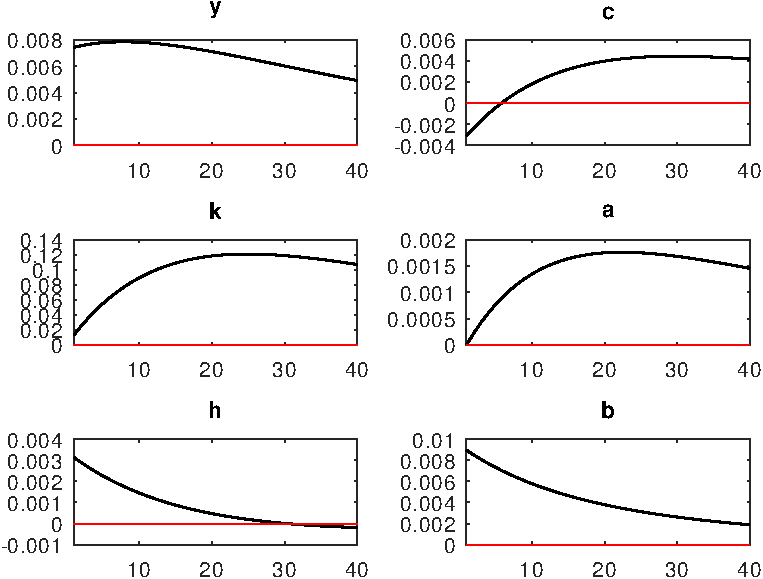
\includegraphics{example1/example1/graphs/example1_IRF_u.pdf}

}

\caption{A figure generated from Dynare software}

\end{figure}

\begin{Shaded}
\begin{Highlighting}[]
\FunctionTok{include\_IRF}\NormalTok{(}\AttributeTok{model=}\StringTok{"example1"}\NormalTok{,}\AttributeTok{IRF =} \StringTok{"u"}\NormalTok{)}

\CommentTok{\# Alternatively, use the path argument }

\FunctionTok{include\_IRF}\NormalTok{(}\AttributeTok{path=}\StringTok{"example1/example1/graphs/example1\_IRF\_u.pdf"}\NormalTok{)}
\end{Highlighting}
\end{Shaded}

However, Dynare figure can only be dynamically included if the output
format is pdf as Dynare produces pdf and eps graphs only.

\hypertarget{the-write_dyn-function}{%
\subsection{6.2 The write\_dyn function}\label{the-write_dyn-function}}

This function writes a new \texttt{dyn} file.

Use \texttt{write\_dyn(code="code",model="someModel")} if you want the
\texttt{Dynare} file to live in the current working directory. if you
want the Dynare file to live in the path different from the current
working directory:

\texttt{write\_dyn(code="code",model="path/to/someDirectory/someModel")}

\begin{Shaded}
\begin{Highlighting}[]
\NormalTok{dynareCodes}\OtherTok{=}\StringTok{\textquotesingle{}var y, c, k, a, h, b;}
\StringTok{varexo e, u;}
\StringTok{parameters beta, rho, alpha, delta, theta, psi, tau;}
\StringTok{alpha = 0.36;}
\StringTok{rho   = 0.95;}
\StringTok{tau   = 0.025;}
\StringTok{beta  = 0.99;}
\StringTok{delta = 0.025;}
\StringTok{psi   = 0;}
\StringTok{theta = 2.95;}
\StringTok{phi   = 0.1;}
\StringTok{model;}
\StringTok{c*theta*h\^{}(1+psi)=(1{-}alpha)*y;}
\StringTok{k = beta*(((exp(b)*c)/(exp(b(+1))*c(+1)))}
\StringTok{          *(exp(b(+1))*alpha*y(+1)+(1{-}delta)*k));}
\StringTok{y = exp(a)*(k({-}1)\^{}alpha)*(h\^{}(1{-}alpha));}
\StringTok{k = exp(b)*(y{-}c)+(1{-}delta)*k({-}1);}
\StringTok{a = rho*a({-}1)+tau*b({-}1) + e;}
\StringTok{b = tau*a({-}1)+rho*b({-}1) + u;}
\StringTok{end;}
\StringTok{initval;}
\StringTok{y = 1.08068253095672;}
\StringTok{c = 0.80359242014163;}
\StringTok{h = 0.29175631001732;}
\StringTok{k = 11.08360443260358;}
\StringTok{a = 0;}
\StringTok{b = 0;}
\StringTok{e = 0;}
\StringTok{u = 0;}
\StringTok{end;}

\StringTok{shocks;}
\StringTok{var e; stderr 0.009;}
\StringTok{var u; stderr 0.009;}
\StringTok{var e, u = phi*0.009*0.009;}
\StringTok{end;}

\StringTok{stoch\_simul;\textquotesingle{}}


\FunctionTok{write\_dyn}\NormalTok{(}\AttributeTok{code=}\NormalTok{dynareCodes, }\AttributeTok{model=}\StringTok{"example1"}\NormalTok{)}

\FunctionTok{write\_dyn}\NormalTok{(}\AttributeTok{code=}\NormalTok{dynareCodes,}\AttributeTok{model=}\StringTok{"DynareR/write\_dyn/example1"}\NormalTok{)}
\end{Highlighting}
\end{Shaded}

\hypertarget{the-write_mod-function}{%
\subsection{6.3 The write\_mod function}\label{the-write_mod-function}}

This function writes a new \texttt{mod} file.

Use \texttt{write\_mod(code="code",model="someModel")} if you want the
\texttt{Dynare} file to live in the current working directory. if you
want the Dynare file to live in the path different from the current
working directory:

\texttt{write\_mod(code="code",model="path/to/someDirectory/someModel")}

\begin{Shaded}
\begin{Highlighting}[]
\NormalTok{DynareCodes}\OtherTok{=}\StringTok{\textquotesingle{}var y, c, k, a, h, b;}
\StringTok{varexo e, u;}
\StringTok{parameters beta, rho, alpha, delta, theta, psi, tau;}
\StringTok{alpha = 0.36;}
\StringTok{rho   = 0.95;}
\StringTok{tau   = 0.025;}
\StringTok{beta  = 0.99;}
\StringTok{delta = 0.025;}
\StringTok{psi   = 0;}
\StringTok{theta = 2.95;}
\StringTok{phi   = 0.1;}
\StringTok{model;}
\StringTok{c*theta*h\^{}(1+psi)=(1{-}alpha)*y;}
\StringTok{k = beta*(((exp(b)*c)/(exp(b(+1))*c(+1)))}
\StringTok{          *(exp(b(+1))*alpha*y(+1)+(1{-}delta)*k));}
\StringTok{y = exp(a)*(k({-}1)\^{}alpha)*(h\^{}(1{-}alpha));}
\StringTok{k = exp(b)*(y{-}c)+(1{-}delta)*k({-}1);}
\StringTok{a = rho*a({-}1)+tau*b({-}1) + e;}
\StringTok{b = tau*a({-}1)+rho*b({-}1) + u;}
\StringTok{end;}
\StringTok{initval;}
\StringTok{y = 1.08068253095672;}
\StringTok{c = 0.80359242014163;}
\StringTok{h = 0.29175631001732;}
\StringTok{k = 11.08360443260358;}
\StringTok{a = 0;}
\StringTok{b = 0;}
\StringTok{e = 0;}
\StringTok{u = 0;}
\StringTok{end;}

\StringTok{shocks;}
\StringTok{var e; stderr 0.009;}
\StringTok{var u; stderr 0.009;}
\StringTok{var e, u = phi*0.009*0.009;}
\StringTok{end;}

\StringTok{stoch\_simul;\textquotesingle{}}


\FunctionTok{write\_mod}\NormalTok{(}\AttributeTok{model=}\StringTok{"example1"}\NormalTok{,}\AttributeTok{code=}\NormalTok{dynareCodes)}

\FunctionTok{write\_mod}\NormalTok{(}\AttributeTok{code=}\NormalTok{dynareCodes,}\AttributeTok{model=}\StringTok{"DynareR/write\_mod/example1"}\NormalTok{)}
\end{Highlighting}
\end{Shaded}

\hypertarget{the-run_dynare-function}{%
\subsection{6.4 The run\_dynare
function}\label{the-run_dynare-function}}

Create and run Dynare \texttt{mod} file

Use this function to create and run Dynare mod file. Use
\texttt{run\_dynare(code="code",model="someModel")} if you want the
Dynare files to live in the current working directory. if you want the
Dynare files to live in the path different from the current working
directory:

\texttt{run\_dynare(code="code",model="path/to/someDirectory/someModel")}

Use \texttt{import\_log=T} argument to return the \texttt{dynare} log
file as list of dataframes in an environment \texttt{dynare}, which can
be accessed via \texttt{dynare\$modelName}.

\begin{Shaded}
\begin{Highlighting}[]
\NormalTok{DynareCodes}\OtherTok{=}\StringTok{\textquotesingle{}var y, c, k, a, h, b;}
\StringTok{varexo e, u;}
\StringTok{parameters beta, rho, alpha, delta, theta, psi, tau;}
\StringTok{alpha = 0.36;}
\StringTok{rho   = 0.95;}
\StringTok{tau   = 0.025;}
\StringTok{beta  = 0.99;}
\StringTok{delta = 0.025;}
\StringTok{psi   = 0;}
\StringTok{theta = 2.95;}
\StringTok{phi   = 0.1;}
\StringTok{model;}
\StringTok{c*theta*h\^{}(1+psi)=(1{-}alpha)*y;}
\StringTok{k = beta*(((exp(b)*c)/(exp(b(+1))*c(+1)))}
\StringTok{          *(exp(b(+1))*alpha*y(+1)+(1{-}delta)*k));}
\StringTok{y = exp(a)*(k({-}1)\^{}alpha)*(h\^{}(1{-}alpha));}
\StringTok{k = exp(b)*(y{-}c)+(1{-}delta)*k({-}1);}
\StringTok{a = rho*a({-}1)+tau*b({-}1) + e;}
\StringTok{b = tau*a({-}1)+rho*b({-}1) + u;}
\StringTok{end;}
\StringTok{initval;}
\StringTok{y = 1.08068253095672;}
\StringTok{c = 0.80359242014163;}
\StringTok{h = 0.29175631001732;}
\StringTok{k = 11.08360443260358;}
\StringTok{a = 0;}
\StringTok{b = 0;}
\StringTok{e = 0;}
\StringTok{u = 0;}
\StringTok{end;}

\StringTok{shocks;}
\StringTok{var e; stderr 0.009;}
\StringTok{var u; stderr 0.009;}
\StringTok{var e, u = phi*0.009*0.009;}
\StringTok{end;}

\StringTok{stoch\_simul;\textquotesingle{}}

\FunctionTok{run\_dynare}\NormalTok{(}\AttributeTok{code=}\NormalTok{DynareCodes,}\AttributeTok{model=}\StringTok{"example1"}\NormalTok{,}\AttributeTok{import\_log =}\NormalTok{ T)}
\FunctionTok{run\_dynare}\NormalTok{(}\AttributeTok{code=}\NormalTok{DynareCodes,}\AttributeTok{model=}\StringTok{"DynareR/run\_dynare/example1"}\NormalTok{)}
\end{Highlighting}
\end{Shaded}

\hypertarget{the-run_models-function}{%
\subsection{6.5 The run\_models
function}\label{the-run_models-function}}

Run multiple existing \texttt{mod} or \texttt{dyn} files.

Use this function to execute multiple existing Dynare files. Use
\texttt{run\_models(model="someModel")} if the Dynare files live in the
current working directory. If the Dynare files live in the path
different from the current working directory:

\texttt{run\_models(model="path/to/someDirectory/someModel")}

Use \texttt{run\_models()} to exectute all the \texttt{dynare} models in
the current working directory. Use
\texttt{run\_models("path/to/someDirectory*)} to run all the
\texttt{dynare} models in \texttt{path/to/someDirectory}.

Where \texttt{agtrend.mod}, \texttt{example1.mod} and
\texttt{example1.mod} are the Dynare model files (with \texttt{mod} or
\texttt{dyn} extension), which live in the current working directory.

\begin{Shaded}
\begin{Highlighting}[]
\FunctionTok{demo}\NormalTok{(agtrend)}
\FunctionTok{demo}\NormalTok{(bkk)}
\FunctionTok{demo}\NormalTok{(example1)}

\CommentTok{\# Provide the list of the \textasciigrave{}Dynare\textasciigrave{} files in a vector}
\CommentTok{\# Ensure that "agtrend.mod", "bkk.mod" and "example1.mod"}
\CommentTok{\# live in the current working directory}

\CommentTok{\# Copy the dynare files to the current working directory}

\FunctionTok{lapply}\NormalTok{(}\FunctionTok{c}\NormalTok{(}\StringTok{"agtrend"}\NormalTok{,}\StringTok{"bkk"}\NormalTok{,}\StringTok{"example1"}\NormalTok{),\textbackslash{}(x) }\FunctionTok{file.copy}\NormalTok{(}\FunctionTok{paste0}\NormalTok{(x,}\StringTok{"/"}\NormalTok{,x,}\StringTok{".mod"}\NormalTok{),}\StringTok{"."}\NormalTok{))}

\FunctionTok{run\_models}\NormalTok{(}\FunctionTok{c}\NormalTok{(}\StringTok{"agtrend"}\NormalTok{,}\StringTok{"bkk"}\NormalTok{,}\StringTok{"example1"}\NormalTok{)) }\CommentTok{\# Run the models in the vector.}
\end{Highlighting}
\end{Shaded}

To run all \texttt{Dynare} models that live in the current working
directory, use the following:

\begin{Shaded}
\begin{Highlighting}[]
\FunctionTok{run\_models}\NormalTok{() }\CommentTok{\# Run all models in Current Working Directory.}
\end{Highlighting}
\end{Shaded}

To run all \texttt{Dynare} models that live in particular path (for
example `DynareR/run\_dynare/' folder), use the following:

\begin{Shaded}
\begin{Highlighting}[]
\CommentTok{\# Copy the dynare files to the \textquotesingle{}DynareR/run\_dynare\textquotesingle{} directory}

\FunctionTok{lapply}\NormalTok{(}\FunctionTok{c}\NormalTok{(}\StringTok{"agtrend"}\NormalTok{,}\StringTok{"bkk"}\NormalTok{,}\StringTok{"example1"}\NormalTok{),\textbackslash{}(x) }\FunctionTok{file.copy}\NormalTok{(}\FunctionTok{paste0}\NormalTok{(x,}\StringTok{".mod"}\NormalTok{),}\StringTok{"DynareR/run\_dynare"}\NormalTok{))}

\FunctionTok{run\_models}\NormalTok{(}\AttributeTok{model =} \StringTok{\textquotesingle{}DynareR/run\_dynare*\textquotesingle{}}\NormalTok{) }\CommentTok{\# notice the * at the end}
\end{Highlighting}
\end{Shaded}

\hypertarget{import_log-function}{%
\section{7 import\_log function}\label{import_log-function}}

This function returns the \texttt{dynare} log output as a list of
dataframes, which include \texttt{summary}, \texttt{shocks},
\texttt{policy}, \texttt{moments}, \texttt{decomposition},
\texttt{correlation} and \texttt{autocorrelation}. The list is
accessible via \texttt{dynare\$modelName}. if the model name is
\texttt{example1}, the policy variables can be obtained via
\texttt{dynare\$example1\$policy} as a dataframe.

\begin{Shaded}
\begin{Highlighting}[]
\FunctionTok{import\_log}\NormalTok{(}\AttributeTok{model=}\StringTok{"example1"}\NormalTok{)}

\FunctionTok{import\_log}\NormalTok{(}\AttributeTok{path=}\StringTok{"example1/example1.log"}\NormalTok{)}

\NormalTok{knitr}\SpecialCharTok{::}\FunctionTok{kable}\NormalTok{(dynare}\SpecialCharTok{$}\NormalTok{example1}\SpecialCharTok{$}\NormalTok{autocorrelation) }
\end{Highlighting}
\end{Shaded}

\hypertarget{set_dynare_version-function}{%
\section{8 set\_dynare\_version
function}\label{set_dynare_version-function}}

On Windows, you can set the version of dynare you want to use. By
default, \texttt{DynareR} package does this for you if the dynare
version ranges from 4.6.1 to 9.9. However, if you are using the
development version of \texttt{dynare}, for example version
\texttt{6-unstable-2022-04-03-0800-700a0e3a}, you can override the
default as follows

\begin{Shaded}
\begin{Highlighting}[]
\FunctionTok{set\_dynare\_version}\NormalTok{(}\StringTok{"6{-}unstable{-}2022{-}04{-}03{-}0800{-}700a0e3a"}\NormalTok{)}
\end{Highlighting}
\end{Shaded}

\hypertarget{set_octave_path-function}{%
\section{9 set\_octave\_path function}\label{set_octave_path-function}}

You can use this function if \texttt{Octave} is not installed in the
standard location.

\begin{Shaded}
\begin{Highlighting}[]
\FunctionTok{set\_octave\_path}\NormalTok{(}\StringTok{\textquotesingle{}C:/Program Files/GNU Octave/Octave{-}6.4.0/mingw64/bin/octave20.exe\textquotesingle{}}\NormalTok{)}
\end{Highlighting}
\end{Shaded}

\hypertarget{add_path-function}{%
\section{10 add\_path function}\label{add_path-function}}

This function is a wrapper of \texttt{addpath} in \texttt{Octave}. If
\texttt{dynare} is not installed in the standard location, use this
function to add the \texttt{matlab} subdirectory. By default,
\texttt{DynareR} does this for if \texttt{dynare} is installed in the
standard location.

\begin{Shaded}
\begin{Highlighting}[]
\FunctionTok{add\_path}\NormalTok{(}\StringTok{\textquotesingle{}/usr/lib/dynare/matlab\textquotesingle{}}\NormalTok{)}\CommentTok{\#  Default for Linux}

\FunctionTok{add\_path}\NormalTok{(}\StringTok{\textquotesingle{}c:/dynare/5.1/matlab\textquotesingle{}}\NormalTok{) }\CommentTok{\# Default for Windows, but 5.1 can change if later version of}
\CommentTok{\# \textasciigrave{}Dynare\textasciigrave{} is installed.}

\FunctionTok{add\_path}\NormalTok{(}\StringTok{\textquotesingle{}/usr/lib/dynare/matlab\textquotesingle{}}\NormalTok{) }\CommentTok{\# Default for macOS}
\end{Highlighting}
\end{Shaded}

\hypertarget{demo}{%
\section{11 Demo}\label{demo}}

The demo files are included and can be accessed via
demo(package=``DynareR'')

\begin{Shaded}
\begin{Highlighting}[]
\FunctionTok{demo}\NormalTok{(run\_dynare)}
\FunctionTok{demo}\NormalTok{(run\_models)}
\FunctionTok{demo}\NormalTok{(import\_log)}
\end{Highlighting}
\end{Shaded}

\hypertarget{template}{%
\section{12 Template}\label{template}}

Template for R Markdown is created. Go to
\texttt{file-\textgreater{}New\ File-\textgreater{}R\ Markdown-\textgreater{}\ From\ Template-\textgreater{}DynareR}.

\hypertarget{similar-packages}{%
\section{Similar packages}\label{similar-packages}}

Similar packages include
\href{https://github.com/sagirumati/EviewsR}{EviewsR}
(\protect\hyperlink{ref-Mati2020a}{Mati, 2020b},
\protect\hyperlink{ref-mati2022eviewsr}{2022b};
\protect\hyperlink{ref-Mati2023}{Mati et al., 2023},
\protect\hyperlink{ref-Mati2024}{2024}),
\href{https://github.com/sagirumati/gretlR}{gretlR}
(\protect\hyperlink{ref-Mati2020b}{Mati, 2020c},
\protect\hyperlink{ref-mati2022gretlr}{2022c}), and
\href{https://github.com/sagirumati/URooTab}{URooTab}
(\protect\hyperlink{ref-Mati2023a}{Mati, 2023b},
\protect\hyperlink{ref-mati2023urootab}{2023a})

For further details, consult Mati
(\protect\hyperlink{ref-Mati2020}{2020a}) and Mati
(\protect\hyperlink{ref-mati2022dynarer}{2022a}).

Please download the example files from
\href{https://github.com/sagirumati/DynareR/tree/master/inst/examples/}{Github}.

\hypertarget{references}{%
\section*{References}\label{references}}
\addcontentsline{toc}{section}{References}

\hypertarget{refs}{}
\begin{CSLReferences}{1}{0}
\leavevmode\vadjust pre{\hypertarget{ref-Mati2020}{}}%
Mati, S. (2020a). DynareR: Bringing the power of dynare to {R, R
Markdown, and Quarto}. \emph{CRAN}.
\url{https://CRAN.R-project.org/package=DynareR}

\leavevmode\vadjust pre{\hypertarget{ref-Mati2020a}{}}%
Mati, S. (2020b). \emph{EviewsR: A seamless integration of {EViews} and
{R}}. \url{https://CRAN.R-project.org/package=EviewsR}

\leavevmode\vadjust pre{\hypertarget{ref-Mati2020b}{}}%
Mati, S. (2020c). \emph{gretlR: A seamless integration of {Gretl} and
{R}}. \url{https://CRAN.R-project.org/package=gretlR}

\leavevmode\vadjust pre{\hypertarget{ref-mati2022dynarer}{}}%
Mati, S. (2022a). \emph{Package {``DynareR''}}.
\url{https://cran.r-project.org/web/packages/DynareR/DynareR.pdf}

\leavevmode\vadjust pre{\hypertarget{ref-mati2022eviewsr}{}}%
Mati, S. (2022b). \emph{Package {``EviewsR''}}.
\url{https://cran.r-project.org/web/packages/EviewsR/EviewsR.pdf}

\leavevmode\vadjust pre{\hypertarget{ref-mati2022gretlr}{}}%
Mati, S. (2022c). \emph{Package {``gretlR''}}.
\url{https://cran.r-project.org/web/packages/gretlR/gretlR.pdf}

\leavevmode\vadjust pre{\hypertarget{ref-mati2023urootab}{}}%
Mati, S. (2023a). \emph{Package {``URooTab''}}.
\url{https://cran.r-project.org/web/packages/URooTab/URooTab.pdf}

\leavevmode\vadjust pre{\hypertarget{ref-Mati2023a}{}}%
Mati, S. (2023b). \emph{{URooTab}: Tabular reporting of {EViews} unit
root tests}. \url{https://github.com/sagirumati/URooTab}

\leavevmode\vadjust pre{\hypertarget{ref-Mati2023}{}}%
Mati, S., Civcir, I., \& Abba, S. I. (2023). {EviewsR}: An r package for
dynamic and reproducible research using {EViews}, r, r markdown and
quarto. \emph{The R Journal}, \emph{15}(2), 169--205.
\url{https://doi.org/10.32614/rj-2023-045}

\leavevmode\vadjust pre{\hypertarget{ref-Mati2024}{}}%
Mati, S., Ismael, G. Y., Masoud, S., Hamad, K. Q., Mohammed, A. A., \&
Hussaini, M. (2024). Revisiting ECOWAS-eurozone exports in the light of
asymmetry. \emph{Cogent Economics \& Finance}, \emph{12}(1), 2309812.
\url{https://doi.org/10.1080/23322039.2024.2309812}

\end{CSLReferences}



\end{document}
